\documentclass{article}[11pt,oneside]
\usepackage{graphicx}

\begin{document}
%Documentation for Seismogram

%% TITLE AND OVERVIEW
\section*{Normal Incidence Reflection Seismogram}
In seismic methods, acoustic energy in the form of pressure or shear waves is input into the ground.
Geophones are used to record the ground motions caused by the acoustic energy. In the case of reflection seismology, we focus on the energy which is reflected off of boundaries that separate layers with different physical properties.

This example allows us to build a synthetic seismogram for a seismic wave which travels vertically. It simulates the case where the source and receiver are coincident and the geologic layers are horizontal. The time taken for the wave to travel from the source and be reflected off of these layers back to the surface depends on the velocity and thickness of each layer.

Synthetic seismograms are routinely generated from well logs (measurements made in depth) and \emph{tied} to the seismic data in order to interpret the seismic data.
Check out: http://library.seg.org/doi/pdf/10.1190/tle33060674.1 for a tutorial.

% TODO: Insert image of normal incidence reflection \& transmission on layers

\section*{Physical Properties}
\subsection*{Density, $\rho$ [kg/m$^3$]}
Density is the mass per unit volume of a material. In general, density increases with depth.

\subsection*{Seismic Velocity, $v$ [m/s]}
Seismic velocities depends on density and elastic properties of the rock. The P or compressional wave velocity is given by
$$v_p = \sqrt{\frac{K + 4/3\mu}{\rho}}$$
and the S or shear wave velocity is given by
$$v_s = \sqrt{\frac{\mu}{\rho}}$$
$K$ and $\mu$ are elastic parameters (the bulk and shear moduli). Most often, seismic velocity increases with depth. What does that imply about the magnitude of the elastic parameters?


\section*{Acoustic Impedance}

Acoustic impedance is the product of density and velocity, $Z_i = \rho_i v_i$.

\section*{Reflectivity}
At an interface energy is partitioned, some is reflected, and some is transmitted. The fraction of amplitude reflected is described by the reflection coefficient:
$$R_i = \frac{Z_{i+1} - Z_i}{Z_{i+1}+Z_i} \quad -1 \leq R_i \leq 1$$
and the amount transmitted is described by the transmission coefficient:
$$T_i = 1-R_i = \frac{2Z_1}{Z_2+Z_1} \quad 0 \leq T_i \leq 2$$

If a seismic wave, with source amplitude 1, is transmitted through the first interface, and reflected off of the second interface, what is the amplitude of the wave that arrives at the geophone?

\begin{figure}[H]
	\centering 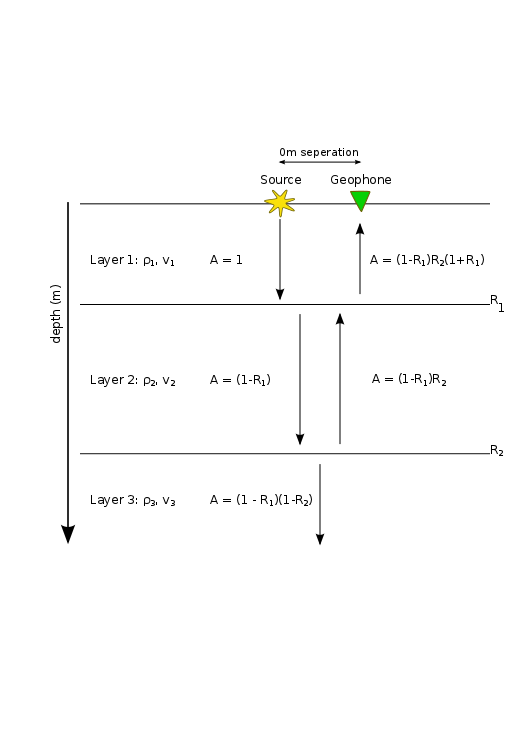
\includegraphics[width=\textwidth]{Amplitude.png}
\end{figure}

What does the polarity of an arrival imply about the physical properties of the layers?


% TODO: talk about polarity (why does it reverse, also which term tends to be more important)
% TODO: Insert image explaining this.

\section*{Depth-Time Curve}
The amount of time taken for the seismic signal to travel from the source to the interface where it is reflected and back to the geophone where it is measured depends on the thickness of the layer and its seismic velocity. The contribution from a single layer with thickness $h_i,$ and velocity $v_i$ is given by
$$t_i = \frac{2h_i}{v_i}$$.

When does the reflection from the second interface arrive?


\begin{figure}[H]
	\centering 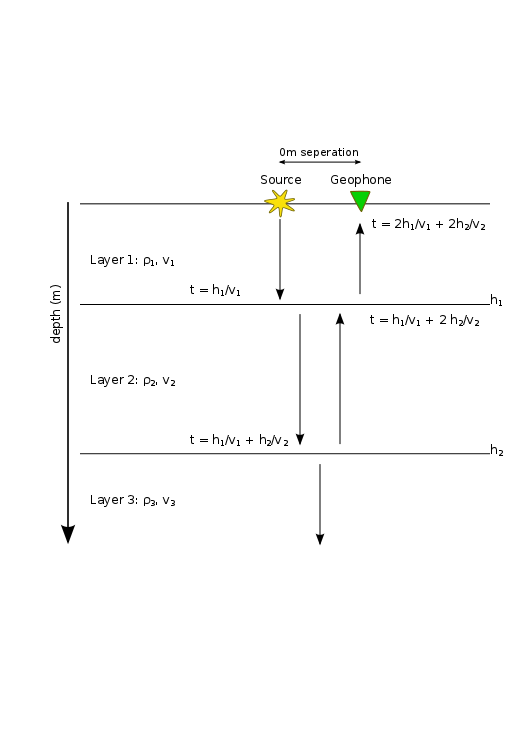
\includegraphics[width=\textwidth]{TimeTravel.png}
\end{figure}
% TODO: Insert image explaining this: show contribution from each layer and the total twt is the sum of all of the contributions.

\section*{Wavelet}
The wavelet is our input energy. Its center frequency ($f$) is related to seismic resolution, which describes how thin a layer can be before reflections from its top and bottom become indistinguishable. The theoretical minimum is $1/4 \lambda$, where $\lambda$ is the wavelength (recall $v = f\lambda$).

\section*{Seismogram}
The reflection seismogram is the convolution of the reflectivity series with the input. The relative amplitude and polarity of the reflection event is given by the reflectivity series (in the absence of attenuation).

\end{document}
